

\begin{savequote}[0.55\linewidth]
	\begin{fancyquote}
		Everyone knows that debugging is twice as hard as writing a program in the
		first place. So if you're as clever as you can be when you write it, how will
		you ever debug it?
	\end{fancyquote}
	\qauthor{Brian W. Kernighan and P. J. Plauger in \\\emph{The Elements of Programming Style}, 1978}
\end{savequote}
\chapter{Testing and verification}\label{ch:testing}
% TODO
% 5. Testing and verification
%    [ Test plans and test results. Unit tests and integration tests.
%      Tools for testing. ]

When testing a system, there are two related procedures that are
used to ensure that the system is working in the intended manner:
verification and validation. Verification is testing whether an
implementation of a model is correctly implemented. This is analogous to
asking  ``did we build it right?''. Validation is checking the accuracy of the model to
a real system. This asks ``was it the right thing to build?''~\autocite{Boehm:1989}.

When testing is done on the whole system to check if the final output makes
sense, this is a kind of validation. This is how the \gls{orionmat} is
currently tested. However, validation testing can not stand on its own. We also
need to improve the system's verification testing. One such way is to implement
unit testing. This kind of testing involves running each unit of the system (such as a function)
and checking if the expected outputs are generated for a given set of inputs.

% TODO describe TDD
By performing unit tests, the expectation of a given unit is recorded in a way
that it can be run repeatedly and in completely automated manner. This allows
for running the same tests both in new environments and whenever a part of the
code changes. Since it is completely automated, debugging in case there are any
unmet expectations can be performed quickly. However, testing can only prove
the existence of bugs, not their absence. This is why a particular form of
software engineering methodology called \acrfull{TDD} advocates
writing tests before the actual code being tested. In this way, the test code
will fail first and just enough code is added to make the test pass. In this way,
it is clear that the added code made that specific test case pass.

Some of examples of tests that are used in the \gls{orionc} code include
\begin{enumerate*}[label={}]
	\enumdescitem{analytic testing} which test numerical
		calculations where an analytic solution is known
		for certain inputs (e.g., the \acrshort{FFT} of
		\(f(x) = \sin 2\pi{}x\));
	\enumdescitem{property testing} which tests if a function
		satisfies certain conditions on its outputs (i.e.,
		a function that outputs data in sorted order can
		be checked to see if the sorted property is
		retained);
	\enumdescitem{integration tests} which test if two
		separate systems can work together (i.e., the
		output of one system can be used as the input to
		another system).
\end{enumerate*}

% TODO explain the floating point testing
% e.g., for float32, ε = 1E-7 tolerance is expected
% What Every Programmer Should Know about Memory <http://www.akkadia.org/drepper/cpumemory.pdf>
% Kahan summation <http://www.drdobbs.com/floating-point-summation/184403224>
% "What Every Computer Scientist Should Know About Floating-Point Arithmetic" <http://docs.sun.com/source/806-3568/ncg_goldberg.html>
It is important to keep in mind that since many of these tests are
performed on floating point data, the tests can not use strict
equality and must compare their values to within a tolerance. For
example, when testing the \acrshort{FFT} implementation, one property that
can be tested is if computing \(\IFourierTrans{\FourierTrans{x}} =
x\). However, due to numerical errors, the absolute error \(\abs{\IFourierTrans{\FourierTrans{x}} -
x}\) is within a range of \(\epsilon = \num{1e-7}\) when
using 32-bit floating point numbers for
computation --- which is expected based on the machine epsilon~\autocite{fftw:accuracy-bench,Tashce:FFT-error}.

\section{Testing portability}

% describe continuous integration and specifically Travis-CI
% explain compiler differences
One of the issues with testing is that some tests that may hold
one machine, may not hold on another. This can be due to
differences in library versions, differences between compilers, or
even differences between processors. This is why testing in
multiple environments is necessary to ensure that the tests are
themselves portable. In order to test in multiple environments,
\gls{orionc} is tested using a continuous integration server which
tests every change on a different machine using different
compilers. Using a continuous integration server like this has
helped track down some issues with using an older version of ITK
and other issues that had to do with how a specific compiler
interpreted the source code.
% explain how TDD and branching and Travis-CI work together
Furthermore, using a continuous integration server allows for a
workflow where every new feature can be worked on separately from
the main ``released'' code and tested as it is being developed.
Only when that code has been appropriately tested will that
feature be brought into the main code. This allows in-progress
code to be worked on separately from working code.

\section{Tracing-based comparison with \gls{orionmat}}

In order to look more closely at whether or not the \gls{orionc}
code implements the same algorithms as \gls{orionmat}, it is
possible to compare the data from across the entire \gls{orionmat}
pipeline. This can be accomplished by recording the input
parameters given to every \gls{orionmat} function and passing
those inputs to the \gls{orionc} input. In \cref{fig:abs-pipe},
the pipeline for \gls{orionc} is depicted on the top row and the
pipeline for \gls{orionmat} is depicted on the bottom row. The
middle row represents the process of taking the \gls{orionmat}
data and passing it to the corresponding \gls{orionc} component.
Then the output of the components in the middle row and the bottom
row are compared. The reason for this comparison procedure is so
that the functions can be compared individually to find where the
two systems deviate instead of having to see the differences
accumulate over the entire system. A full description of the
algorithm is given in
\cref{alg:mat-trace-data,alg:mat-trace-compare}. In
\cref{alg:mat-trace-compare}, the algorithm makes reference to an
``appropriate method''. This method depends on the kind of data being
compared. For example, in \cref{tbl:compare-Makefilter}, the
comparison is done by generating a histogram \(a\) and \(b\) for
each volume so that both histograms contain the same number of
bins \(n\) and the same bin boundaries. Then the intersection of the two
histograms is calculated as
\begin{equation}
 K_{\cap}(a, b) = \sum_{i = 1}^{n} min( a_i, b_i ).
\end{equation}

\begin{sidewaysfigure}
	\centering
	  % Cases
	  \definecolor{inputcol}{RGB}{255,255,255}
	  \definecolor{lgray}{RGB}{255,255,255}
	  \definecolor{ngray}{RGB}{255,255,255}
	  \definecolor{dgray}{RGB}{255,255,255}

	  \definecolor{tcol}{RGB}{0,0,0}
	  % Cases
	  \definecolor{lblue}{RGB}{102,102,255}
	  \definecolor{nblue}{RGB}{51,51,255}
	  \definecolor{dblue}{RGB}{0,0,255}
	\resizebox{1.0\linewidth}{!}{%\documentclass[tikz, border=10pt]{standalone}
\tikzset{
    vertex/.style = {
        circle,
        fill            = black,
        outer sep = 2pt,
        inner sep = 1pt,
    }
}

%\begin{document}

\newcommand{\myfun}[2] {$fun^{#1}_{#2}$}
  
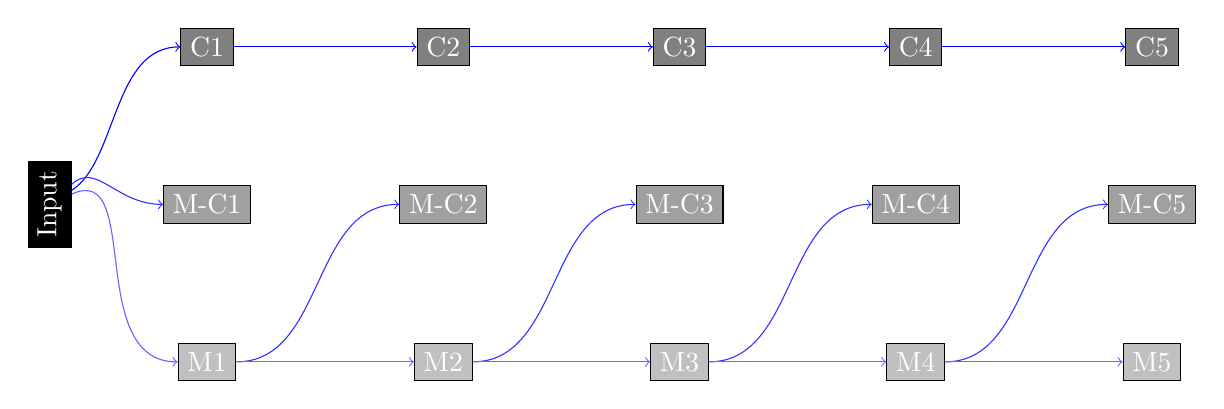
\begin{tikzpicture}
  % Cases
  \definecolor{lgray}{RGB}{192,192,192}
  \definecolor{ngray}{RGB}{160,160,160}
  \definecolor{dgray}{RGB}{128,128,128}
  % Cases
  \definecolor{lblue}{RGB}{102,102,255}
  \definecolor{nblue}{RGB}{51,51,255}
  \definecolor{dblue}{RGB}{0,0,255}
% Input node
\node[draw,fill=black,text=white,rotate=90] (Input) at (2,2) {Input};  
  
% Matlab nodes
\node[draw,fill=lgray,text=white] (funM1) at ( 4,0) {\myfun{M}{1}};
\node[draw,fill=lgray,text=white] (funM2) at ( 7,0) {\myfun{M}{2}};
\node[draw,fill=lgray,text=white] (funM3) at (10,0) {\myfun{M}{3}};
\node[draw,fill=lgray,text=white] (funM4) at (13,0) {\myfun{M}{4}};
\node[draw,fill=lgray,text=white] (funM5) at (16,0) {\myfun{M}{5}};

% MC nodes
\node[draw,fill=ngray,text=white] (funMC1) at ( 4,2) {\myfun{M-C}{1}};
\node[draw,fill=ngray,text=white] (funMC2) at ( 7,2) {\myfun{M-C}{2}};
\node[draw,fill=ngray,text=white] (funMC3) at (10,2) {\myfun{M-C}{3}};
\node[draw,fill=ngray,text=white] (funMC4) at (13,2) {\myfun{M-C}{4}};
\node[draw,fill=ngray,text=white] (funMC5) at (16,2) {\myfun{M-C}{5}};

% C nodes
\node[draw,fill=dgray,text=white] (funC1) at ( 4,4) {\myfun{C}{1}};
\node[draw,fill=dgray,text=white] (funC2) at ( 7,4) {\myfun{C}{2}};
\node[draw,fill=dgray,text=white] (funC3) at (10,4) {\myfun{C}{3}};
\node[draw,fill=dgray,text=white] (funC4) at (13,4) {\myfun{C}{4}};
\node[draw,fill=dgray,text=white] (funC5) at (16,4) {\myfun{C}{5}};


% Initial data conection
\draw[->,draw=dblue] (Input) to[in=180,out=0] (funC1);
\draw[->,draw=nblue] (Input) to[in=180,out=0] (funMC1);
\draw[->,draw=lblue] (Input) to[in=180,out=0] (funM1);

% C
\draw[->,draw=dblue] (funC1) to[in=180,out=0] (funC2);
\draw[->,draw=dblue] (funC2) to[in=180,out=0] (funC3);
\draw[->,draw=dblue] (funC3) to[in=180,out=0] (funC4);
\draw[->,draw=dblue] (funC4) to[in=180,out=0] (funC5);

% MC
\draw[->,draw=nblue] (funM1) to[in=180,out=0] (funMC2);
\draw[->,draw=nblue] (funM2) to[in=180,out=0] (funMC3);
\draw[->,draw=nblue] (funM3) to[in=180,out=0] (funMC4);
\draw[->,draw=nblue] (funM4) to[in=180,out=0] (funMC5);

% M
\draw[->,draw=lblue] (funM1) to[in=180,out=0] (funM2);
\draw[->,draw=lblue] (funM2) to[in=180,out=0] (funM3);
\draw[->,draw=lblue] (funM3) to[in=180,out=0] (funM4);
\draw[->,draw=lblue] (funM4) to[in=180,out=0] (funM5);


\end{tikzpicture}

\begin{tikzpicture}
  % Dialectics
  \node[draw] (Thesis) at (0,0) {Thesis};
  \node[draw,fill=black,text=white] (Antithesis) at (2.3,0) {Antithesis};
  \node[draw,fill=gray,text=white] (Synthesis) at (1,2) {Synthesis};
  
  \draw node[vertex] (Joint) at (1,0) {};
  
  \draw[-,draw=blue] (Thesis) to (Joint);
  \draw[-,draw=blue] (Antithesis) to (Joint);
  \draw[->,draw=blue] (Joint) to (Synthesis);
  \draw[->,draw=blue] (Synthesis) to[in=180,out=180] (Thesis);
  
  \node at (1.0, -1.0) {\textit{a) Dialectics}};
  
  % Opposition
  \node[draw] (ArgumentA) at (5,0) {Argument};
  \node[draw,fill=black,text=white] (ArgumentB) at (7.5,0) {Opposition};
  
  \draw[->,draw=blue] (ArgumentA) to (ArgumentB);
  
  \node at (6., -1.0) {\textit{b) Opposition}};
  
  % Innovation
  \node[draw] (ArgumentA) at (10.1,0) {Argument};
  \node[draw,fill=black,text=white] (ArgumentB) at (13,0) {Opposition};
  \node[draw,fill=yellow] (ArgumentC) at (12,2) {Innovation};
  
  \draw node[vertex] (Joint) at (11.5,0) {};
  
  \draw[-] (ArgumentA) to (Joint);
  \draw[-] (ArgumentB) to (Joint);
  \draw[->,draw=blue] (Joint) to (ArgumentC);
  
  \node at (11.5, -1.0) {\textit{c) Innovation}};
\end{tikzpicture}
%\end{document}}
	\caption{Abstract diagram of pipeline of both \gls{orionc}
		and \gls{orionmat}}\label{fig:abs-pipe}
\end{sidewaysfigure}

\begin{algorithm}
	\caption{MATLAB tracing data capture}\label{alg:mat-trace-data}
	\begin{algorithmic}[1]
		\State Set breakpoints at every \gls{orionm} function start and end.
		\State Run the MATLAB code under the debugger.
		\While{ \gls{orionm} Program has not finished }
			\State When the debugger stops, save the $State$ of the input and output data at
				each breakpoint along with a stack frame
				ID. Add $State$ to $SavedStates$.
			\State Continue the debugger.
		\EndWhile
	\end{algorithmic}
\end{algorithm}

\begin{algorithm}
	\caption{MATLAB tracing data comparison}\label{alg:mat-trace-compare}
	\begin{algorithmic}[1]
		\State \Input $SavedStates \gets$ the list of all saved
		states from \cref{alg:mat-trace-data}.
		\For{$State \in SavedStates$}
			\State Load the MATLAB data from $State$.
			\State Convert MATLAB data structures to C
			data structures.
			\State Call corresponding \gls{orionc}
				function using C data structures
			\State Compare the results using an
				appropriate method.
		\EndFor
	\end{algorithmic}
\end{algorithm}

\begin{table}
	\centering
	\begin{tabular}{cc}
		\toprule
		\be{}Stack ID     & \be{} histogram intersection \\
		\midrule
		1 & 0.999973665203964 \\
		2 & 0.999967508148729 \\
		3 & 0.999978416844418 \\
		4 & 0.999982131154914 \\
		5 & 0.999959276433577 \\
		\bottomrule
	\end{tabular}
	\caption{Example of comparison captured from data for the
		\computertext{Makefilter} function}\label{tbl:compare-Makefilter}
\end{table}


